\chapter{Esercizi}

\section{Esercizi venerdi 13/03/2026}
\begin{figure}[H]    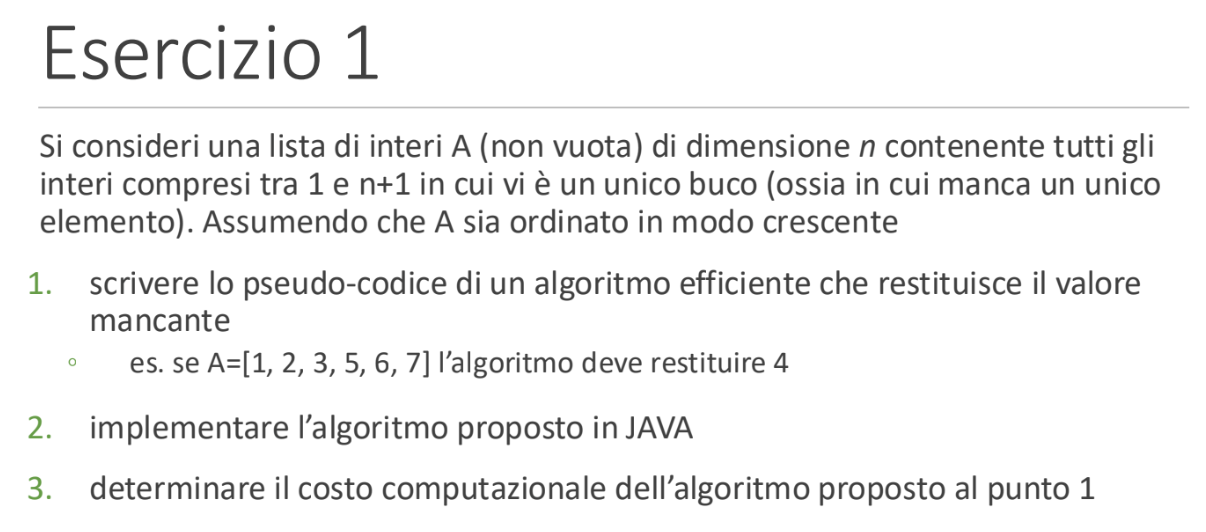
\includegraphics[width=0.75\linewidth]{../images/Screenshot 2026-03-13 alle 10.15.09.png}
    \label{fig:placeholder}
\end{figure}

\noindent \textbf{1.}\\
\begin{verbatim}
    Trova_buco(A,i,j)
        if(A[i] != i e |A| > 1)
            return i
        if(A[j] = j e |A| > 1)
            return j+1
        if(|A|=1)
            if(A[i] != i)
                return 1
            else return 2
        q = punto medio tra i e j
        if q = A[q]
            Trova_buco(q+1,j)
        else
            Trova_buco(i,q)
\end{verbatim}
\noindent All'inizio mi trovo on i=1 e j=7, nel primo if controllo se c'è il buco nel primo elemento e lo restituisco. Nel secondo if controllo se c'è il buco nell'ultimo elemento.\\
\begin{figure}[H]
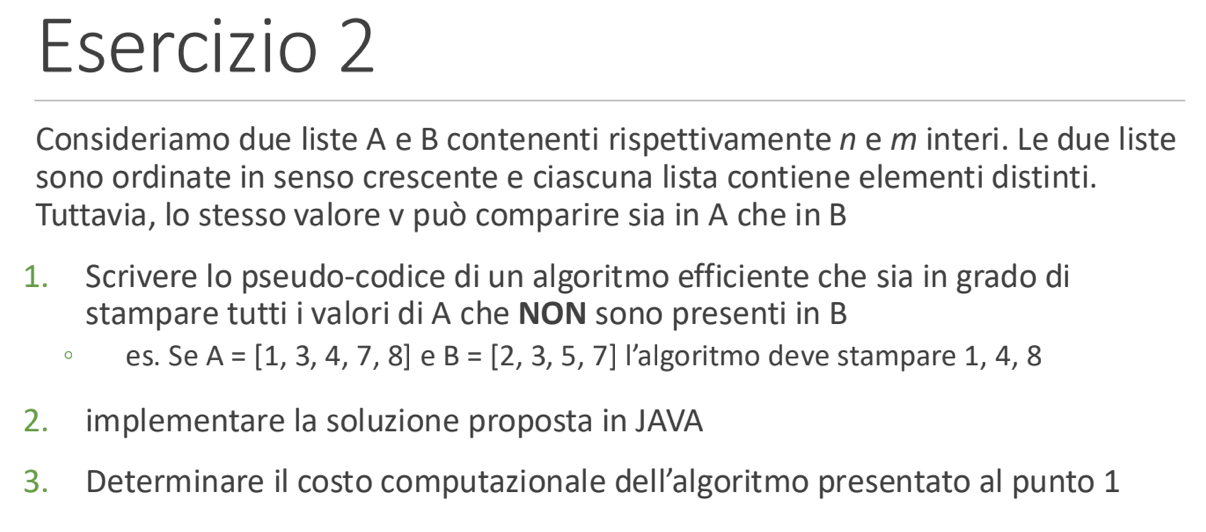
\includegraphics[width=0.75\linewidth]{../images/Screenshot 2026-03-13 alle 10.45.07.png}
    \label{fig:placeholder}
\end{figure}
\noindent \textbf{1.}
$$A = [1, 3, 4, 7, 8] \text{ con } |A| = n$$
$$B = [2, 3, 5, 7] \text{ con } |B| = m$$
Procedura merge-sort, uso indice $i$ per $A$ e $j$ per $B$:

\begin{verbatim}
    A = [1, 3, 4, 7, 8]
         ^  
         |        
         i
         
    B = [2, 3, 5, 7]
         ^  
         |        
         j
         
\end{verbatim}
\noindent Questo è lo pseudocodice:
\begin{verbatim}
i = 1
j = 1
while (i <= n AND j <= m)
    if(A[i] < B[j])
        stampo(A[i])
        i = i + 1
    else if (A[i] > B[j])
            j = j + 1
        else 
            i = i + 1
            j = j + 1
while(i <= n)
        stampo A[i]
        i = i + 1 
\end{verbatim}
da correggere per quando ci sono i duplicati in $A$\\
Costo algoritmo $n + m$\\
Se non era ordinato comunque aveva un vantaggio prima ordinare le due liste e poi applicare il merge invece di fare la ricerca binaria
\begin{figure}[H]
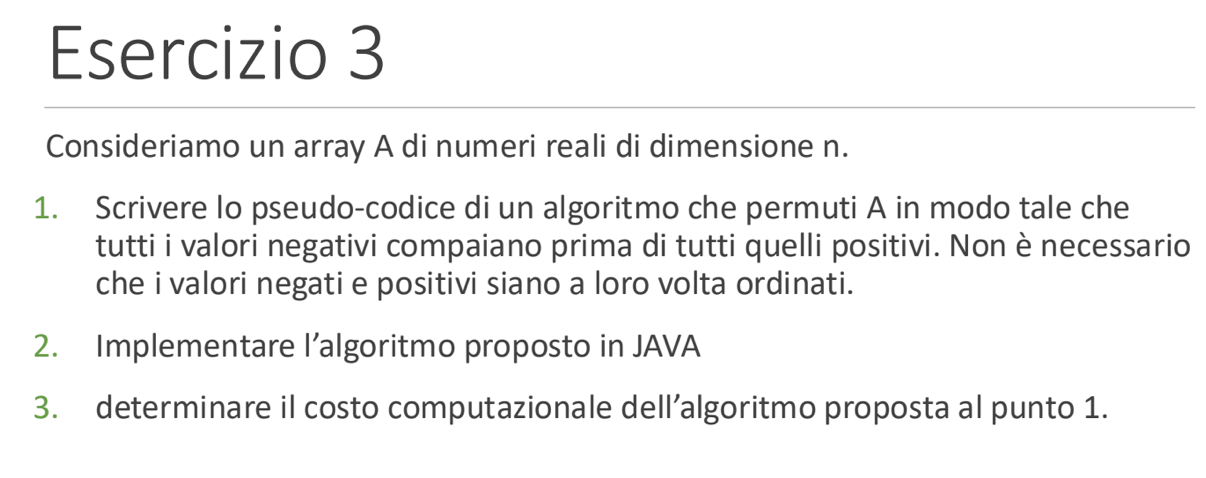
\includegraphics[width=0.75\linewidth]{../images/Screenshot 2026-03-13 alle 11.14.01.png}
    \label{fig:placeholder}
\end{figure}
\noindent \textbf{1.}\\
In qeusto caso usiamo Quick sort con pivot=0.\\
\begin{verbatim}
    A = [-1, 7, 15, -3, 2, 8, -10]
       ^ ^ 
       | |      
       i j
\end{verbatim}
\begin{verbatim}
    A = [-1, 7, 15, -3, 2, 8, -10]
         ^ 
         |      
        j,i
\end{verbatim}
\begin{verbatim}
    A = [-1, 7, 15, -3, 2, 8, -10]
         ^           ^
         |           |
         i           j
\end{verbatim}
\noindent pseudocodice
\begin{verbatim}
while(j <= |A|)
    if(A[j] < 0)
        swap(A[i+1], A[j])
        i++
    j++
\end{verbatim}
\section{prova}
ciao ciao ciao.